% -*- mode: LaTeX; mode: TeX-PDF; coding: utf-8  -*-

% Пусть $h=(h_1,h_2),\ h_1,h_2>0,\ r\in\mathbb{N}^2,\ S_{h,r}(f)$ --- среднее В.~А.~Стеклова функции $f$ двух переменных,
% $m \in \mathbb{N},\ E$ --- тождественный оператор.
% В работе получена оценка 
% отклонений
% обобщенных средних В.~А.~Стеклова 
% $$
% S_{h,r,m}(f)=(E-(E-S_{h,r})^m)(f), 
% $$
% для $2m$ раз непрерывно дифференцирумых функций двух переменных.
% Библиография: 6 назв.


В дальнейшем $\mathbb{R},\ 
\mathbb{R}_+,
\ \mathbb{Z}_+,
\ \mathbb{N}$ ---
соответственно множества вещественных, 
вещественных неотрицательных, 
целых неотрицательных, натуральных
чисел.
Если $A$ --- некоторое множество, то $A^n=A\times\ldots \times A$ ($n$ раз);
Если $a\in\mathbb{R}$, то $\mathbf{a}^n=(a,\ldots,a)$.
% $\mathbf{0}^n=(0,\ldots,0)$ --- нулевой элемент $\mathbb{R}^n,$
% $\mathbf{1}^n=(1,\ldots,1)$ ($n$ единиц). 
Пусть рассматривается некоторая величина $x\in\mathbb{R}^n,$ тогда
$x_k$ ($k=1,\ldots,n$) обозначает ее $k$-ю координату. 
% Если $x,\ y \in \mathbb{R}^n,$ то
% скалярное произведение элементов $x,\ y$ и норма $x$ определяются равенствами 
% $$
% (x,y)=\sum_{k=1}^n x_ky_k,\qquad |x|=\sqrt{(x,x)}.
% $$
Пусть $a,\ b \in \mathbb{R}^n,$ тогда запись $a\leqslant b$ ($a<b$) означает, что 
$a_k\leqslant b_k$ ($a_k<b_k$) при каждом $k=1,\ldots,n,\ ab=(a_1b_1,\ldots,a_n b_n)$,
$\lfloor{a}\rfloor=(\lfloor{a_1}\rfloor,\ldots,\lfloor{a_n}\rfloor)$,
$\overline{a}=\prod_{i=1}^n a_i$, 
если дополнительно $b_k\neq 0$ ($k=1,\ldots, n$), то $a/b=(a_1/b_1,\ldots,a_n/ b_n)$.  
Пусть $a\in \mathbb{Z}^n$, $b\in \mathbb{N}^n$, тогда $a \bmod b =(a_1 \bmod b_1,\ldots,a_n \bmod b_n)$.
Если $a,\ b \in \mathbb{Z}^n,\ a\leqslant b,$ то $[a:b]$ --- множество точек
$x\in \mathbb{Z}^n$, удовлетворяющих неравенствам $a\leqslant x \leqslant b$.

% Пусть $G \subset \mathbb{R}^n,$ через $C(G)$    
% обозначаем множество непрерывных функций
% $f:G\to\mathbb{R},$ 
% \begin{equation*}
%   \|f\|_{G,\infty}=\sup_{x\in G}|f(x)|;
% \end{equation*}
% если $f$ измерима на $G,\ 1\leqslant p < \infty,$ то полагаем 
% \begin{equation*}
%   \|f\|_{G,p}=\left(\int_{G}|f|^p\right)^{1/p}.
% \end{equation*}
% В дальнейшем $C^{(r)}(G)$ --- множество функций имеющих все частные производные порядка не выше $r,$ непрерывные на $G,$ где
% $r\in \mathbb{Z}_+,\   G$ открыто ($G\subset\mathbb{R}^2$).
% Пусть
% $f \in C^{(r)}(G),\ 
% x\in G,$ $1\leqslant p \leqslant \infty,$
% обозначим
% \begin{equation*}
%   \mathcal{D}_{r}f(x) =  \sqrt{\sum_{k=0}^{r}C_{r}^{k} \left(\frac{\partial^{r} f(x)}{\partial x_1^{k} \partial x_2^{r-k}}\right)^2}.
% \end{equation*}
% Если $a,b\in\mathbb{R}^2,\ a<b,\ z\in\mathbb{R}_{+}^{2}$ такое, что $[a-z,b+z]\subset G,\ f \in C^{(2m)}(G)$ ($m\in\mathbb{N}$), то 
% \begin{equation*}
%  \Lambda_{z,m}^*(f,[a,b])_p=\sup_{u\in[-z,z]}\|\mathcal{D}_{2m}f\|_{[a+u, b+u],p}.
% \end{equation*}


% Если $f\in C(\mathbb{R}),\ h>0,\ r-1 \in \mathbb{N},\ x \in \mathbb{R},$ то 
% \begin{align*}
%   &S_{h,1}(f,x)=\frac{1}{h}\int_{-h/2}^{h/2} f(x+t)\,dt,\\
%   &S_{h,r}(f,x)=S_{h,1}(S_{h,r-1}(f),x).
% \end{align*}
% Функция $S_{h,r}(f)$ называется средним В.~А.~Стеклова  порядка $r$ с шагом $h$ функции~$f.$  

Положим при $t\in\mathbb{R}$, $h>0$, $r\in\mathbb{N}$
\begin{align*}
  \psi_r(t)&=
  \begin{cases}
    \frac{1}{(r-1)!}\sum\limits_{0\leqslant k<\left(|t|+\frac{r}{2}\right)}(-1)^kC_r^k\left(|t|+\frac{r}{2}-k\right)^{r-1},
    &\ \text{если}\ |t|\leqslant r/2,\\
    0,&\ \text{если}\ |t| > r/2,
  \end{cases}\\
  % \psi_{h,r}(t)&=\frac{1}{h}\psi_r\left(\frac{t}{h}\right).
  \psi_{h,r}(t)&=\psi_r\left(\frac{t}{h}\right).
\end{align*}

Если $t\in\mathbb{R}^n,\  h>\mathbf{0}^n,\ r\in\mathbb{N}^n,$ то
\begin{equation*}
  \psi_{h,r}(t)=\prod_{k=1}^n\psi_{h_k,r_k}(t_k).
\end{equation*}
% Для функций двух
% переменных среднее В.~А.~Стеклова определяется следующим образом 
% \begin{equation*}
%   S_{h,r}(f)=S_{h_1,r_1}S_{h_2,r_2}(f). 
% \end{equation*}
% При этом равенство понимается 
% так:
% сначала оператор $S_{h_1,r_1}$ применяется к $f$ как функции одного первого
% аргумента, а затем оператор $S_{h_2,r_2}$ применяется к $S_{h_1,r_1}(f)$ как функции одного второго
% аргумента.

% Через $E$  обозначаем тождественный оператор.

%%%%%%%%%%%%%%%%%%%%%%%%%%%%%%%%%%%%%%%%%%%%%%%%%%%%%%%%%%%%%%%%%%%%%%%%%%%%%%%%%%%%%%%%%
Пусть известны значения  функции $\varphi$, принадлежащей некоторому классу гладкости, 
в  узлах $\{u^{(k)}=kh\}$ ($k\in [\mathbf{0}^n : K-\mathbf{1}^n]$, $K\in \mathbb{N}^n$,
$h>\mathbf{0}^n$) прямоугольной
равномерной сетки. 
Сетку с известными значениями в узлах будем называть \textit{крупной сеткой}.

Необходимо приближённо найти неизвестные значения
функции $\varphi$ между заданными узлами.

Считаем что, узлы
$ \{v^{(m)}=mt\}$,  ($m\in [\mathbf{0}^n : M-\mathbf{1}^n]$,
$M\in \mathbb{N}^n$, $t>\mathbf{0}^n$), 
в которых требуется найти значения, 
также расположены
равномерно.
Такую  систему узлов %сетку размером %$M = N(K-1) + K$
будем называть
\textit{мелкой сеткой}.
% Обозначим для удобства $N^* = N+1$.
%В этих обозначениях количество узлов мелкой сетки $M = N^* (K-1) + 1$.

Будем считать, что крупная сетка является подмножеством мелкой сетки и
%выполнено соотношение
%$M = N(K-1) + 1$, $N\in\mathbb{N}^n$.
$N\in\mathbb{N}^n$ такое, что $N-\mathbf{1}^n$ узлов мелкой сетки содержится строго между
смежными узлами крупной сетки.

Множество из $\overline{N}$ точек мелкой сетки, содержащееся между узлами крупной будем называть
\textit{ячейкой}.

На рисунке~\ref{fig:net_common} приведён пример крупной и мелкой сеток
для случая $n=2$.
\begin{figure}[h!]
  \centering
  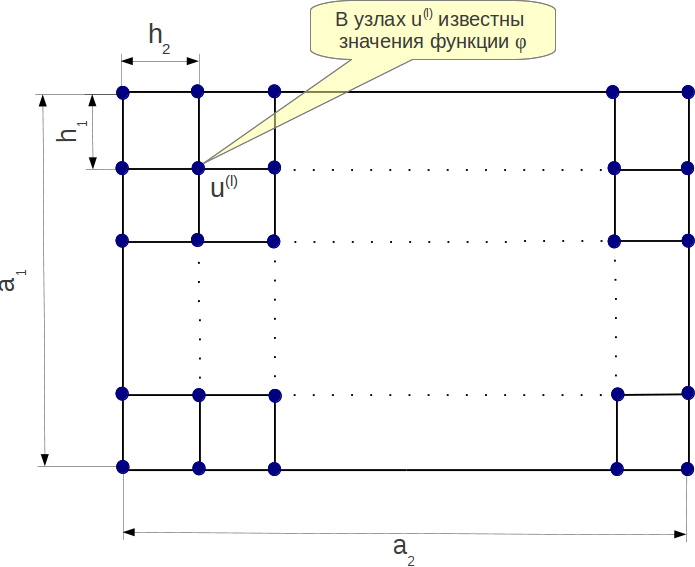
\includegraphics{net_2D}
  \caption{Постановка задачи}
  \label{fig:net_common}
\end{figure}
%\FloatBarrier


%%% Local Variables: 
%%% mode: latex
%%% TeX-master: "paper_func_recv"
%%% End: 

